\documentclass[10pt]{beamer}
\usepackage{amsmath, graphicx, textcomp,multirow,subfigure, verbatim}

\usetheme{Rochester}
%\usetheme{PaloAlto}
\setbeamertemplate{footline}{\insertframenumber/\inserttotalframenumber}

\newcommand{\true}{{\mbox{\hspace*{0cm}\tiny{\sf true}} }}
\newcommand{\means}{{\mbox{\hspace*{0cm}\tiny{\sf means}} }}
\newcommand{\logit}{\ensuremath{\mbox{logit}}}

\title{Statistical Analysis of Structural MRI Data}
\author{John Muschelli, Elizabeth Sweeney, Russell Shinohara, Ani Eloyan and Ciprian Crainiceanu }

\begin{document}

\frame{\titlepage}
 
 
  
 
\frame{
	\frametitle{Setup}
	
Before this course begins... 
	
\begin{enumerate} 
\item Install R (http://cran.r-project.org)
\item Install R Studio (http://www.rstudio.com)
\item Open R Studio and install devtools package in R: 
\begin{semiverbatim}

>install.packages(`devtools')

>library(devtools)

>install\_github(?muschellij2/ENARSC2015?)

\end{semiverbatim}
\end{enumerate} 	


}


 
 
 
\frame{
	\frametitle{Setup}
	
Once ENARSC2015 installs, run...
	
\begin{semiverbatim}
> library(ENARSC2015)

> copy\_data(OUTPUTDIRECTORY)

\# where OUTPUTDIRECTORY is the output directory you want data
\#  to be copied to.  All analysis will be done in this directory.


\end{semiverbatim}


}



\frame{
	\frametitle{Course Deliverables}

\begin{enumerate}	
\item Knowledge of  fslR in R 
\begin{enumerate}
\item Interactively explore data with the imaging software Medical Image Processing, Analysis, and Visualization (MIPAV)
\item Image preprocessing with MIPAV
\item Reading, writing, plotting and manipulation of imaging data in R
\end{enumerate} 
\end{enumerate} 

}

\frame{
	\frametitle{Course Deliverables}

Subtract the a follow-up T1-w volume from a baseline T1-w volume. 

\begin{figure}
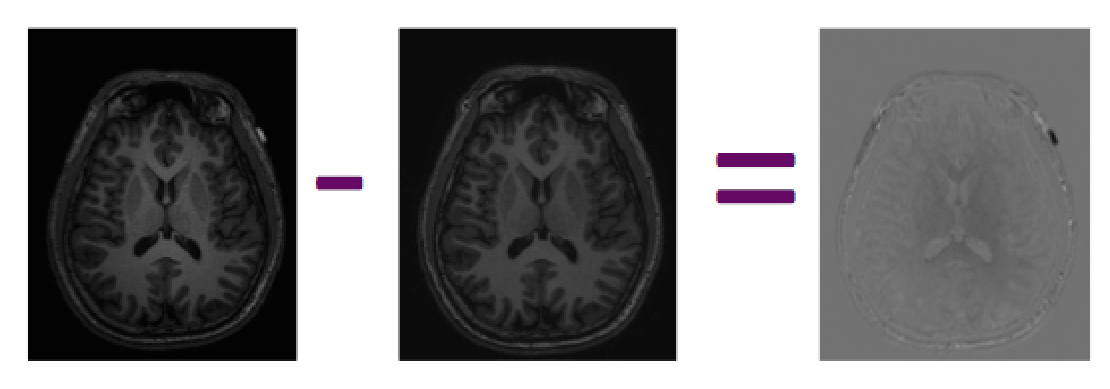
\includegraphics[width=1\linewidth]{subtraction.png}
\end{figure} 


}

\frame{
	\frametitle{Course Deliverables}

Perform a template-based analysis. 

\begin{figure}
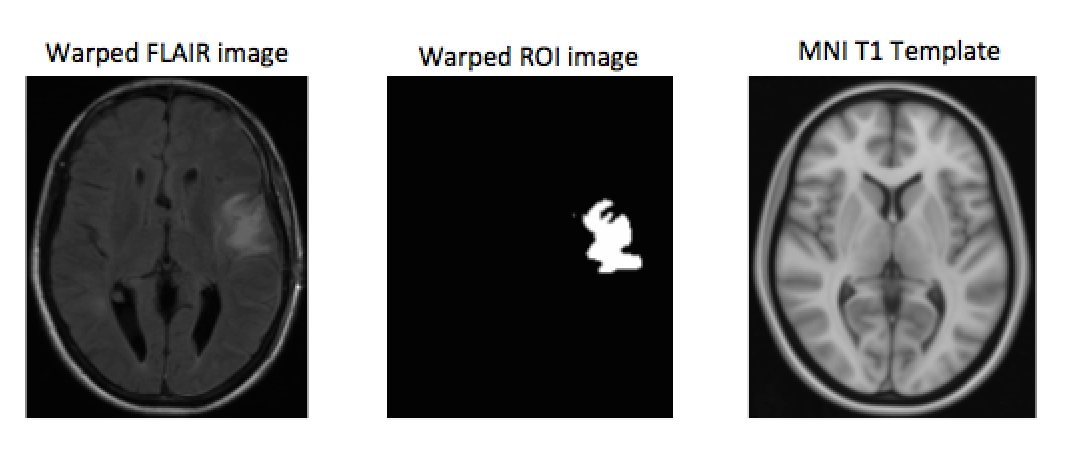
\includegraphics[width=1\linewidth]{template.png}
\end{figure} 


}

\frame{
	\frametitle{Outline}

\begin{enumerate} 
\item Structural MRI Data
\item Public MRI Data
\item Opening Images in R
\item Image Preprocessing
\item fslr and ANTsR: R packages for Image preprocessing
\item Image Pre-processing in R with fslr 
\item Image Analysis in R

\end{enumerate}

}


\frame{
	\frametitle{Structural MRI Data}
	
(A1) Fluid-attenuated inversion recovery (FLAIR)

(A2) T2-weighted (T2-w) 

(A3) Proton density (PD) 

(A4) T1-weighted (T1-w)


\begin{figure}
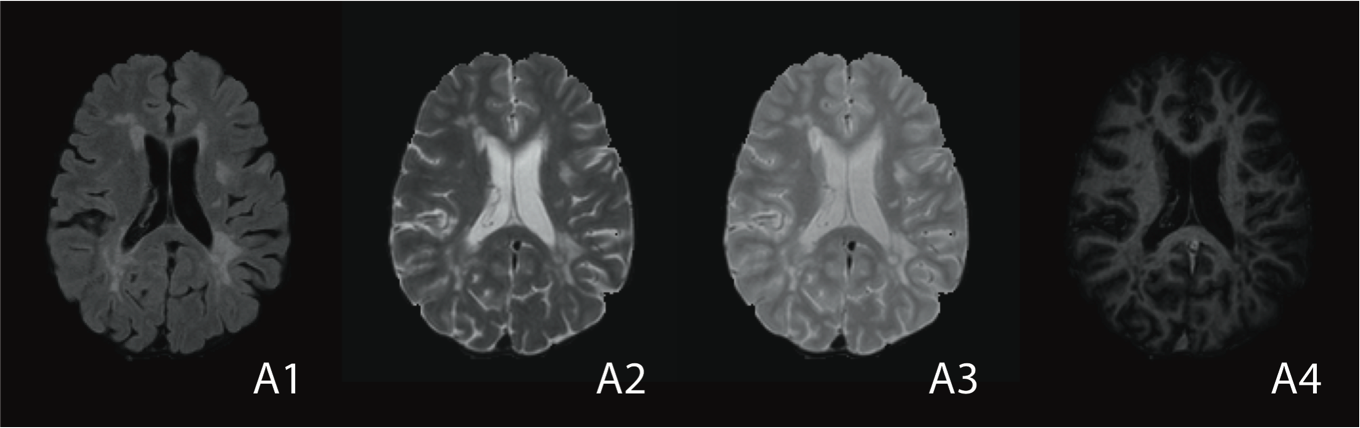
\includegraphics[width=.8\linewidth]{Modalities.png}
\end{figure} 


}


\frame{
	\frametitle{Structural MRI Data}
	
MRI Signal Intensities

\begin{figure}
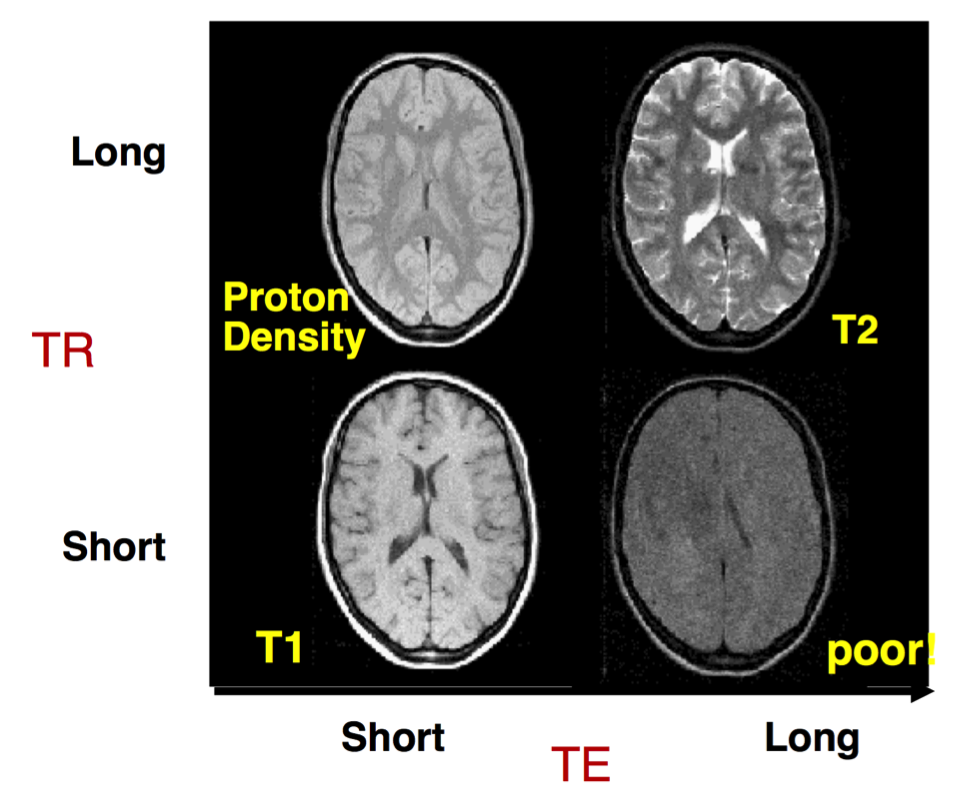
\includegraphics[width=.5\linewidth]{sequences.png}
\end{figure} 

Slide borrowed with permission from Martin Lindquist 


}


\frame{
	\frametitle{Structural MRI Data}
	
MRI Signal Intensities

\begin{figure}
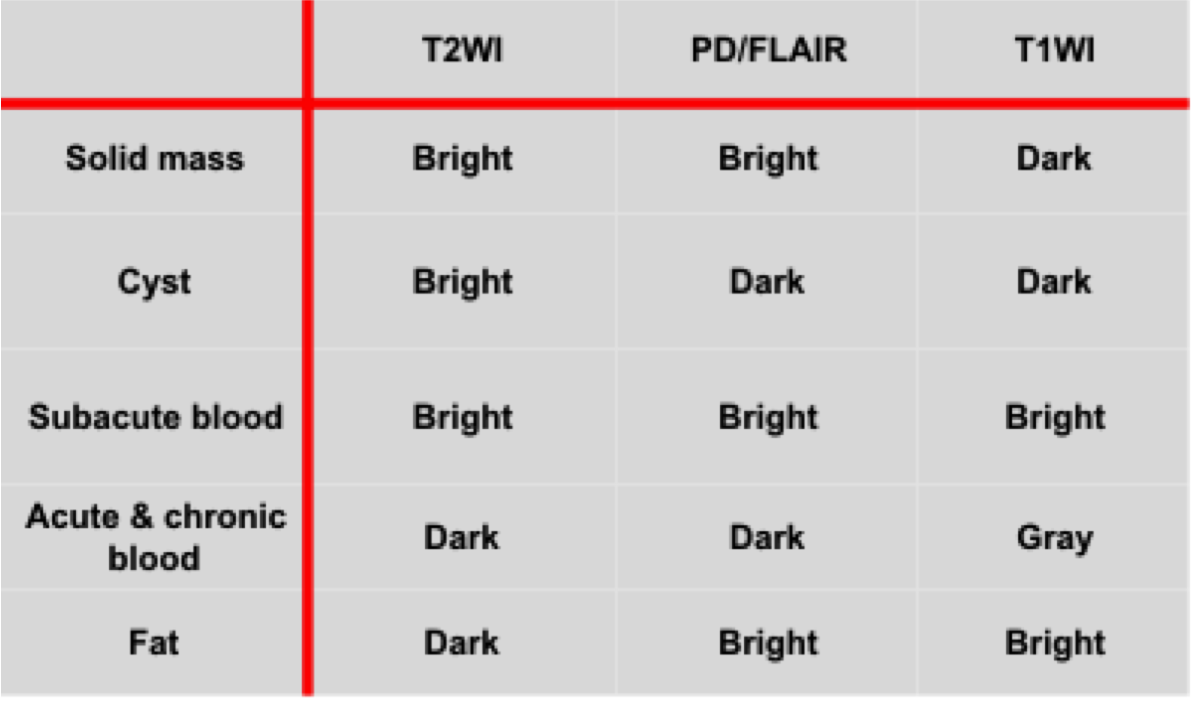
\includegraphics[width=.5\linewidth]{sequences2.png}
\end{figure} 



}

\end{document}